\documentclass[a4paper,12pt]{article}
\usepackage[utf8]{inputenc}
\usepackage[T1]{fontenc}
\usepackage[italian]{babel}
\usepackage{graphicx}
\usepackage{geometry}
\usepackage{csquotes}

\usepackage{fancyhdr}
\usepackage[hidelinks]{hyperref}
\usepackage{booktabs}
\usepackage{listings}
\usepackage{xcolor}
\usepackage{float}
\usepackage{longtable}
\usepackage{tabularx}
\usepackage[all]{nowidow}
\usepackage[backend=biber,style=numeric]{biblatex}

\addbibresource{refs.bib}

% Configurazione margini
\geometry{
	a4paper,
	total={170mm,257mm},
	left=20mm,
	top=20mm,
}

% Configurazione per il codice
\lstset{
	basicstyle=\ttfamily\small,
	breaklines=true,
	frame=single,
	backgroundcolor=\color{gray!10},
	keywordstyle=\color{blue},
	stringstyle=\color{red},
	commentstyle=\color{green!50!black},
	showstringspaces=false
}

% Activate fancy page style
\pagestyle{fancy}

% Clear default headers and footers
\fancyhf{}

% Create footer line and remove header line
\renewcommand{\headrulewidth}{0 px}
\renewcommand{\footrulewidth}{0.2 px}

% Configurazione maketitle
\title{\textbf{HAIVE}}
\author{an AI for the bug-themed strategy game}
\date{\today}

\nocite{*}

\begin{document}

	% --- FRONTESPIZIO ---
	\begin{titlepage}

		\noindent
		\begin{minipage}[c]{0.25\textwidth}
			
\includegraphics[width=0.8\linewidth]{logo_unisa.pdf} 
		\end{minipage}
		\hfill 
		\begin{minipage}[c]{0.75\textwidth}
			\centering 
			{\LARGE \textsc{Università degli Studi di Salerno}} \\
			\vspace{2mm} 
			{\small \textbf{Corso di Fondamenti di Intelligenza Artificiale (FIA)}} \\
			\vspace{1mm}
			{\normalsize Anno Accademico 2025/26}
		\end{minipage}
		
		\centering
		\vspace{1cm}

    	\begin{figure}[hbt!]
			\centering
			
\includegraphics[width=0.3\textwidth]{logo.png} 
			\maketitle
		\end{figure}

		\vspace{1cm}
		
		\begin{tabular}{l r}
			\textbf{Autore} & \textbf{Matricola} \\
			\hline
			Forte Guglielmo & 0512119526 \\
			Rega Maristella & 0512119032 \\
			Russo Serena & 0512119098 \\
			Squitieri Andrea & 0512119008 \\
		\end{tabular}

		\vspace{2cm}
		\textbf{LINK GITHUB:} \url{https://github.com/andrea-sq/hAIve}

		\thispagestyle{empty}
	\end{titlepage}
	
	% --- HEADER + FOOTER SETUP ---
	
	\fancyfoot[L]{HAIVE}
	\fancyfoot[R]{G. Forte, M. Rega, S. Russo, A. Squitieri\hspace{2mm} \textbf{\thepage}}

	% --- SOMMARIO / INDICE ---
	\tableofcontents
	\newpage
	
	% --- CONTENUTO ---
	
	\section{Introduzione}

	\textit{Hive} è un gioco da tavolo strategico per due giocatori, ideato da John Yanni e pubblicato nella prima edizione nel 2001.

	Rientra nei giochi deterministici ad informazione perfetta e a somma zero, tuttavia, a differenza di esempi più celebri come il gioco degli scacchi, non possiede una plancia e può essere svolto su qualsiasi superficie piana.\\
	In seguito alla più recente espansione, il numero totale di pezzi è 28, 
	di cui 14 neri e 14 bianchi, raffiguranti un insieme di insetti, aracnidi e isopodi, ognuno con un modo particolare di muoversi.
	L'obiettivo è catturare l'\textit{ape regina} avversaria, facendo sì che sia completamente circondata da altri pezzi.

	\textbf{Perché Hive?} Un'analisi del branching-factor \cite{ai_for_hive} mostra che, negli stadi più avanzati del gioco, il fattore di ramificazione è stabile a 60. 
	Pertanto, la crescita esponenziale di Hive è circa due volte quella degli scacchi, il cui fattore di ramificazione è intorno al 30.\\
	L'interesse nel creare un'intelligenza artificiale in grado di giocare ad Hive non deriva solo dall'elevata complessità, ma anche dalla scarsa notorietà del gioco che lo rende un problema non ancora esplorato esaustivamente. 

	\section{Descrizione del problema}
		\subsection{Obiettivi}
		\subsection{Specifiche PEAS}
		\subsection{Analisi del problema}
		
		Le due principali regole che ogni pezzo deve rispettare sono:
		\begin{itemize}
			\item \textit{One Hive Rule}: i pezzi in gioco devono essere costantemente connessi, non è mai possibile dividere l'alveare in due o più parti;\\
			\begin{center}
			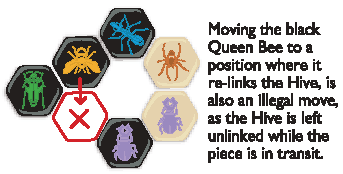
\includegraphics[width=0.5\linewidth]{onehive.pdf} 
			\end{center}
			\item \textit{Freedom To Move}: poichè le creature si muovono scorrendo intorno all'alveare, un pezzo può muoversi da o verso una posizione solo se può fisicamente scivolare in quella direzione.\\
			Fanno eccezione a questa regola Grillo, Coleottero, Coccinella, ed eventualmente Zanzara, che possono muoversi sopra l'alveare.\\
			\begin{center}
			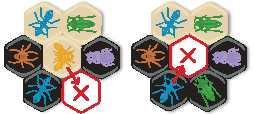
\includegraphics[width=0.5\linewidth]{freedomtomove.pdf} 
			\end{center}		
		\end{itemize}

	\section{Soluzioni proposte}
		\subsection{Minimax}
		\subsection{Reinforcement Learning}

	\section{Conclusioni finali}

	\printbibliography

\end{document}
